\section{R\'ESUM\'E CONSOLID\'E PUBLIC}
\label{sec:resume}

\subsection{Résumé consolidé public en français}
\underline{Analyse d'Images d'Observation de la Terre Multi-Modales}.

Le projet MAESTRIA vise à résoudre des challenges méthodologiques relatifs à l’analyse automatique de très grands volumes d’images acquises par des plateformes d’Observation de la Terre (OT). Plus spécifiquement, MAESTRIA vise à générer des cartes d’occupation et usage des sols à l’échelle nationale, à de multiples résolutions spatiales et sémantiques, à partir d’images satellitaires multi-modales et multi-temporelles. L’objectif final est de fournir un panel large de produits d’occupation des sols qui soit exploitable autant à des échelles locales que nationales et autant pour des besoins de politiques publiques que pour la modélisation scientifique (e.g., climat, planification urbaine, suivi des cultures, détection et évaluation des changements). L’objectif de MAESTRIA est alors de développer des méthodes qui cherchent à exploiter de manière optimale les images d’OT multi-sources pour être en capacité de produire des cartes d’occupation des sols à très large échelle spatiale et avec des résolutions spatiales très variables. Le projet MAESTRIA se place dans un cadre de recherche ouverte et reproductible : codes sources et cartes générées sont mises à disposition de manière libre.

\subsubsection*{Titre 2 : précise les méthodes ou technologies utilisées (150 caractères max espaces compris)}

\ANRinfo{Le paragraphe 2 indique comment les résultats attendus sont obtenus grâce à certaines méthodes ou/et technologies. Les technologies utilisées ou/et les méthodes permettant de surmonter les verrous sont explicitées (il faut éviter le jargon scientifique, les acronymes ou les abréviations).}


\subsubsection*{Résultats majeurs du projet (environ 600 caractères espaces compris)}

\ANRinfo{Faits marquants diffusables en direction du grand public, expliciter les applications ou/et les usages rendus possibles, quelles sont les pistes de recherche ou/et de développement originales, éventuellement non prévues au départ.\\
Préciser aussi toute autre retombée= partenariats internationaux, nouveaux débouchés, nouveaux contrats, start-up, synergies de recherche, pôles de compétitivité, etc.}


\subsubsection*{Production scientifique et brevets depuis le début du projet}(environ 500 caractères espaces compris) \\
\ANRinfo{Ne pas mettre une simple liste mais faire quelques commentaires. Vous pouvez aussi indiquer les actions de normalisation}


\subsubsection*{Illustration}
\begin{figure}[h]
    \centering
    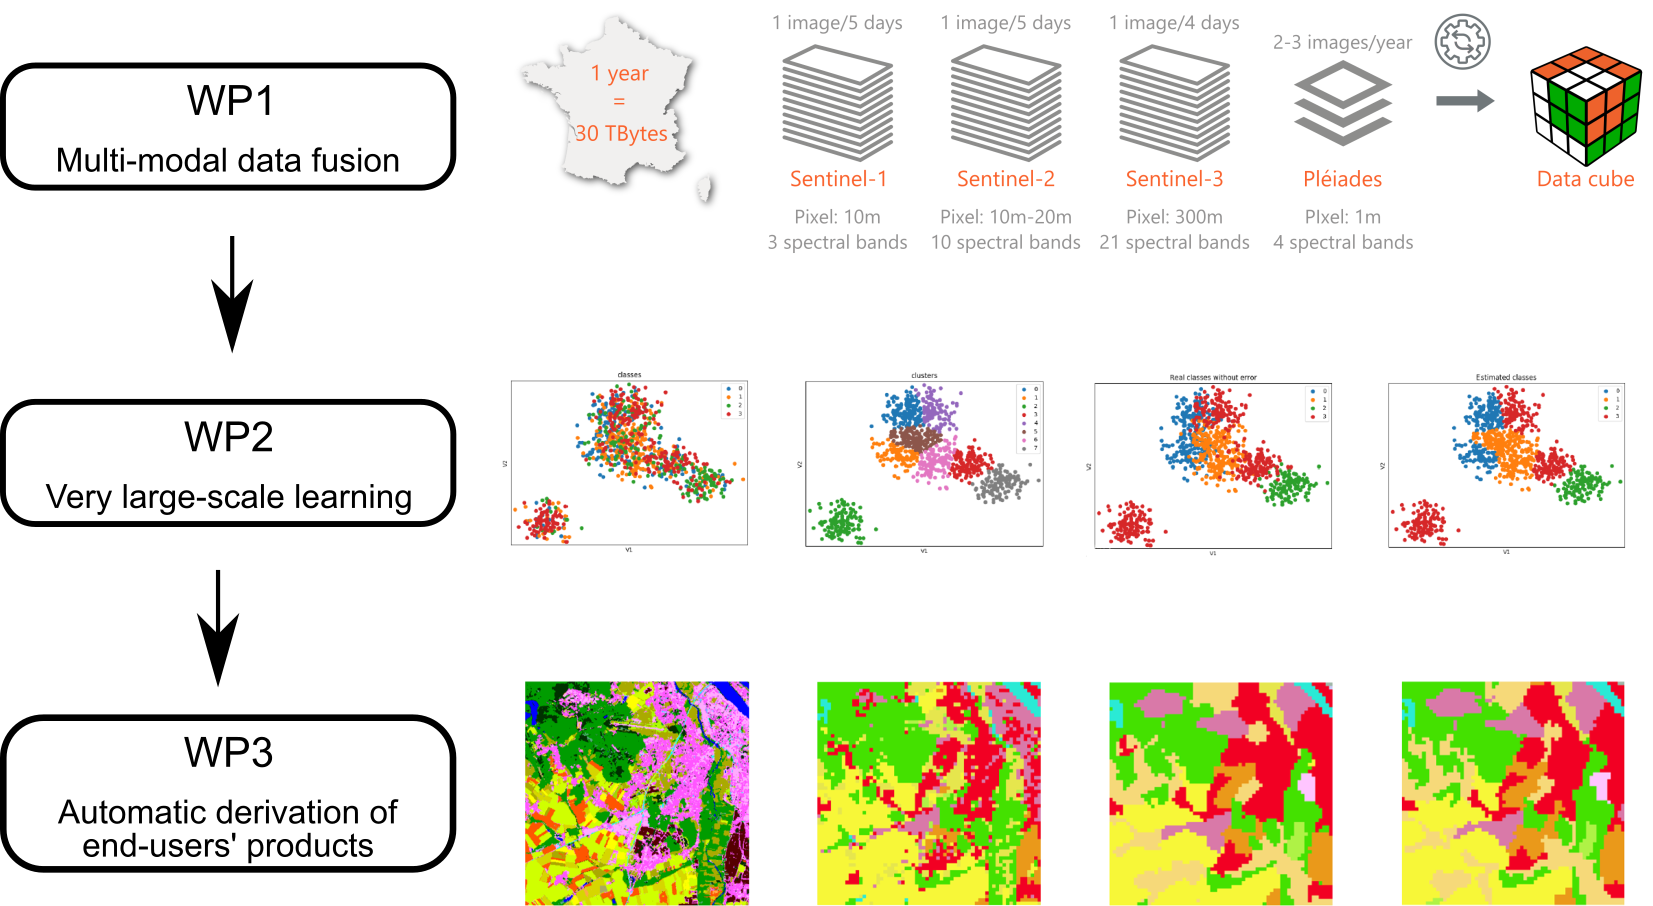
\includegraphics[width=0.9\columnwidth]{img/wp_maestria.png}
    \caption{Architecture of the MAESTRIA project. From raw EO data to on-purpose land-cover maps.}
    \label{fig:enter-label}
\end{figure}



\subsubsection*{Informations factuelles}

Le projet ANR MAESTRIA est un projet de recherche fondamentale coordonné par Clément Mallet (LASTIG) conjointement avec le CESBIO. Le projet a commencé en octobre 2019 et a duré 54 mois. Il a bénéficié d’une aide ANR de 568$\:$k€ pour un coût global de l’ordre de \textcolor{red}{??}$\:$k€. Il a reçu le soutien du pôle de compétitivité Aerospace Valley.


\subsection{Résumé consolidé public en anglais}

The MAESTRIA project aims to solve methodological challenges related to the automatic analysis of a very large amount of images acquired by Earth Observation (EO) platforms. More specifically, MAESTRIA aims to generate national-scale land-cover and land-use maps, at multiple spatial and semantic resolutions, from multi-modal and multi-temporal satellite images. The ultimate aim is to provide a wide range of land-cover/land-use products that can be exploited at both local and national scales, and for both public policy needs and scientific modelling (e.g., climate, urban planning, crop monitoring, change detection and monitoring). The aim of MAESTRIA is therefore to develop methods that leverage
current challenges in multisource Earth Observation image analysis
 to produce land-cover/land-use maps at very large spatial scales and with highly variable spatial resolutions. The MAESTRIA project is grounded on an open and reproducible research policy: source codes and generated maps are made freely available.